\documentclass[a4paper, 12pt]{article}
\usepackage{listings} 
\usepackage{xcolor}
\usepackage{mdframed}
\usepackage{graphicx}
\usepackage{pgfplots}
\usepackage{float}
\usepackage{mathtools}

%% Custom FSM's
\usepackage{tikz}
\usetikzlibrary{automata, positioning, arrows, circuits.logic.US}
\tikzset{thick, ->, >=stealth', node distance=6cm, every state/.style={thick, fill=gray!10}, initial text=$ $}
\tikzstyle{intersection}=[circle, fill=black, inner sep=0pt, minimum size=1.5mm]

%% Macros for logic timing diagrams
\newcounter{wavenum}
\setlength{\unitlength}{1cm}
% advance clock one cycle, not to be called directly
\newcommand*{\clki}{
  \draw (t_cur) -- ++(0,.3) -- ++(.5,0) -- ++(0,-.6) -- ++(.5,0) -- ++(0,.3)
    node[time] (t_cur) {};
}
\newcommand*{\bitvector}[3]{
  \draw[fill=#3] (t_cur) -- ++( .1, .3) -- ++(#2-.2,0) -- ++(.1, -.3)
                         -- ++(-.1,-.3) -- ++(.2-#2,0) -- cycle;
  \path (t_cur) -- node[anchor=mid] {#1} ++(#2,0) node[time] (t_cur) {};
}
% \known{val}{length}
\newcommand*{\known}[2]{
    \bitvector{#1}{#2}{white}
}
% \unknown{length}
\newcommand*{\unknown}[2][XXX]{
    \bitvector{#1}{#2}{black!20}
}
% \bit{1 or 0}{length}
\newcommand*{\bit}[2]{
  \draw (t_cur) -- ++(0,.6*#1-.3) -- ++(#2,0) -- ++(0,.3-.6*#1)
    node[time] (t_cur) {};
}
% \unknownbit{length}
\newcommand*{\unknownbit}[1]{
  \draw[ultra thick,black!50] (t_cur) -- ++(#1,0) node[time] (t_cur) {};
}
% \nextwave{name}
\newcommand{\nextwave}[1]{
  \path (0,\value{wavenum}) node[left] {#1} node[time] (t_cur) {};
  \addtocounter{wavenum}{-1}
}
% \clk{name}{period}
\newcommand{\clk}[2]{
    \nextwave{#1}
    \FPeval{\res}{(\wavewidth+1)/#2}
    \FPeval{\reshalf}{#2/2}
    \foreach \t in {1,2,...,\res}{
        \bit{\reshalf}{1}
        \bit{\reshalf}{0}
    }
}

% \begin{wave}[clkname]{num_waves}{clock_cycles}{start_val}
\newenvironment{wave}[4][clk]{
  \begin{tikzpicture}[draw=black, yscale=.7,xscale=1]
    \tikzstyle{time}=[coordinate]
    \setlength{\unitlength}{1cm}
    \def\wavewidth{#3}
    \setcounter{wavenum}{0}
    \nextwave{#1}
    \foreach \t in {0,1,...,\wavewidth}{
    	 \pgfmathtruncatemacro{\val}{\t+#4} %Calculate time values
      \draw[dotted] (t_cur) + (0,.5) node[above] {\tiny{t=\val}} -- ++(0,.4-#2);
      \clki
    }
}{\end{tikzpicture}}

% Specific Line Breaks
% See https://tex.stackexchange.com/questions/26174/ for details
\usepackage[british]{babel} 

% Page Margins
\usepackage[margin=1.00in]{geometry}

% Large, array-sized, ceiling and floor operators
\DeclarePairedDelimiter\ceil{\lceil}{\rceil}
\DeclarePairedDelimiter\floor{\lfloor}{\rfloor}
\definecolor{code-gray}{gray}{0.93}

% Beginning of Document
\begin{document}
% Title
\title{ECE 440 - Homework \#6}
\author{Collin Heist}
\date{\today}
\maketitle

% Table of Content and Listings
\pagenumbering{arabic}

% Beginning of Report
\section{Problem 1}
\begin{figure}[H]
\centering
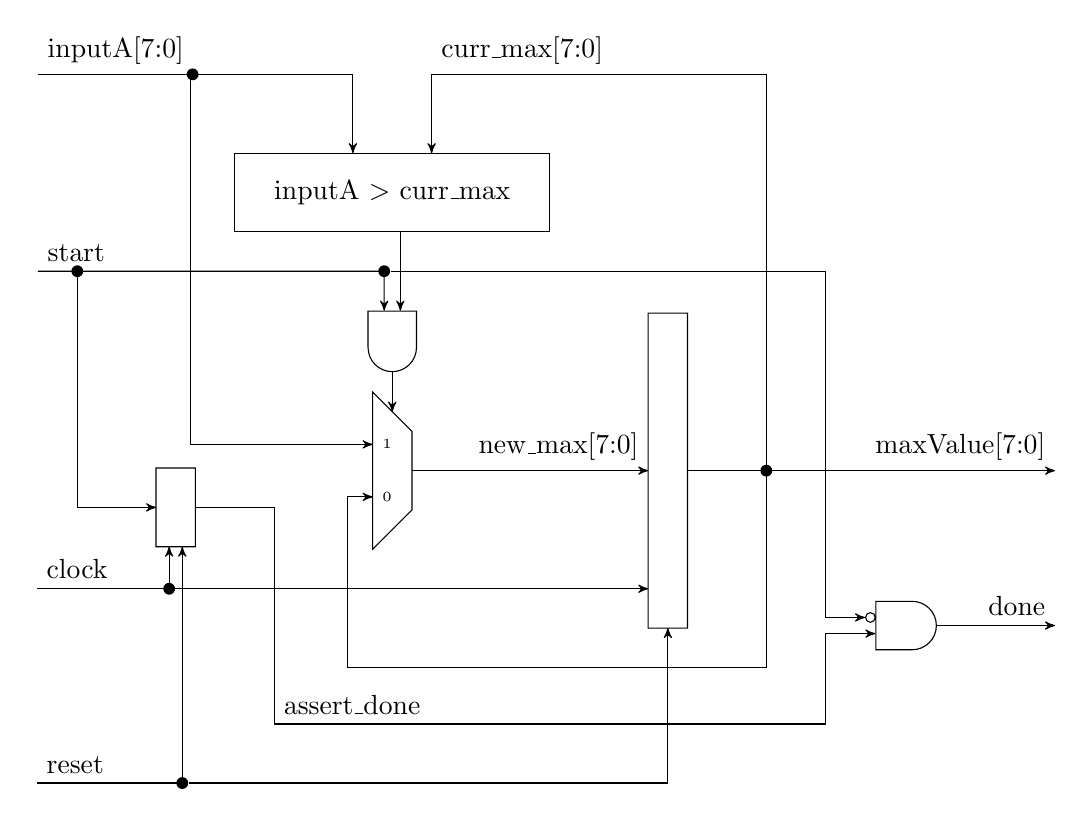
\begin{tikzpicture}[circuit logic US]
\draw (-1, 0) node (inputA-text) [above right] {inputA[7:0]} -- (1, 0) node (inputABranch) [xshift=-1pt, intersection] {} -- (3, 0) -- (3, -1);
\draw (1.5, -1) rectangle (5.5, -2) node[midway] {inputA $>$ curr\_max};
\node[and gate, rotate=-90, anchor=west] (and1) at (3.5, -3) {};
\draw[<-] (and1.input 1) -- ++(0, 1) {};
\draw[<-] (and1.input 2)  -- ++(0, 0.5) node (startBranch2) [intersection] {} -- (-0.5, -2.5) node (startBranch) [intersection] {} -- ++(-0.5, 0) node (start) [above right] {start};
\draw (and1.output) -- ++(0, -0.5) node (and1End) {};
\draw (and1End) -- ++(0.25, -0.25) -- ++(0, -0.5) node (muxOut) {} -- ++(0, -0.5) -- ++(-0.5, -0.5) -- ++(0, 2/3) node (mux0) [right] {\tiny{0}} -- ++(0, 2/3) node (mux1) [right] {\tiny{1}} -- ++(0, 2/3) -- cycle;
\draw[<-] (mux1) -- ++(-2.5, 0) node (temp) {} -- (temp |- inputABranch);
\draw (muxOut.center) -- ++(3, 0) node (FFin-text) [above left] {new\_max[7:0]} node (FFin) {};
\draw (FFin.center) -- ++(0, 2) -- ++(0.5, 0) -- ++(0, -2) node (FFout) {} -- ++(0, -2) -- ++(-0.25, 0) node (FFreset) {} -- ++(-0.25, 0) -- ++(0, .5) node (FFclock) {} -- cycle;
\draw (FFout.center) -- ++(1, 0) node (FFoutBranch) [intersection] {} -- (FFoutBranch |- inputABranch) -- (4, 0) node [above right] (currMax) {curr\_max[7:0]} -- ++(0, -1);
\draw (FFoutBranch.center) -- +(0, -2.5) node (temp) {} -- (mux1 |- temp) -- ++(-0.5, 0) node (temp) {} -- (temp |- mux0) -- (mux0);
\draw (startBranch.center) -- ++(0, -3) -- ++(1, 0) node (FF1) {};
\draw (FF1) -- ++(0, 0.5) -- ++(0.5, 0) -- ++(0, -0.5) node (FF1out) {} -- ++(0, -0.5) -- ++(-0.5/3, 0) node (FF1resetIn) {} -- ++(-0.5/3, 0) node (FF1clockIn) {} -- ++(-0.5/3, 0) -- cycle;
\node[and gate, inputs=in] (and2) at (10, -7) {};
\draw (FF1out.center) -- ++(1, 0) -- ++(0, -2.75) node (temp) [above right] {assert\_done} -- ++(7, 0) node (temp) {} -- (temp |- and2.input 2) -- (and2.input 2);
\draw (startBranch2) -- (temp |- startBranch2) node (temp) {} -- (and2.input 1 -| temp) -- (and2.input 1);
\draw (and2.output) -- ++(1.5, 0) node (temp) {} node (doneText) [above left] {done};
\draw (FFoutBranch.center) -- (FFoutBranch -| temp) node (maxValueText) [above left] {maxValue[7:0]};
\draw[<-] (FFclock.center) -- (FFclock.center -| start) -- ++(-0.5, 0) node (temp) {} node (clock) [above right] {clock};
\draw[<-] (FF1clockIn.center) -- (FF1clockIn |- FFclock) node (clockBranch) [intersection] {};
\draw[<-] (FF1resetIn.center) -- ++(0, -3) node (resetBranch) [intersection] {} -- (temp.center |- resetBranch) node (reset) [above right] {reset};
\draw (resetBranch) -- (FFreset.center |- resetBranch) -- (FFreset.center);
\end{tikzpicture}
\end{figure}

\end{document}